\documentclass[11pt,a4paper]{article}

% ─── packages ────────────────────────────────────────────────────────────────
\usepackage[utf8]{inputenc}
\usepackage[T1]{fontenc}
\usepackage{lmodern}
\usepackage[a4paper,margin=2.3cm]{geometry}
\usepackage{graphicx}
\usepackage{amsmath,amssymb}
\usepackage{booktabs}
\usepackage{array}
\usepackage{xcolor}
\usepackage{tikz}
\usetikzlibrary{shapes.geometric,arrows.meta,positioning,calc,fit,backgrounds}
\usepackage[hidelinks]{hyperref}
\usepackage{caption}
\usepackage{subcaption}
\usepackage{enumitem}
\usepackage{fancyhdr}
\usepackage{titlesec}

% \result{region}{value} — prints the value; lets us swap in real numbers later.
\newcommand{\result}[2]{#2}

\definecolor{brain}{RGB}{34,94,168}
\definecolor{accent}{RGB}{197,27,50}
\definecolor{enc}{RGB}{220,237,250}
\definecolor{dec}{RGB}{255,235,220}
\definecolor{bott}{RGB}{225,245,225}

\pagestyle{fancy}\fancyhf{}
\rhead{\small BraTS-PED 2026 — Task 2}
\lhead{\small Pediatric Brain Tumour Segmentation}
\cfoot{\thepage}
\setlength{\headheight}{14pt}

\titleformat{\section}{\large\bfseries\color{brain}}{\thesection}{0.6em}{}
\titleformat{\subsection}{\normalsize\bfseries}{\thesubsection}{0.6em}{}

% ─── title ───────────────────────────────────────────────────────────────────
\title{\vspace{-1.0cm}\textbf{\color{brain}A Skull-Stripped, Residual-Encoder nnU-Net Ensemble with
Lesion-Wise Post-Processing for Pediatric Brain Tumour Segmentation}\\[0.3cm]
\large BraTS-PED 2026 Challenge (Task 2) --- Technical Report}
\author{ujjwalbaid0408\\\small Pediatric Brain Tumour Segmentation Project}
\date{June 2026}

\begin{document}
\maketitle
\thispagestyle{fancy}

% =============================================================================
\begin{abstract}
\noindent
Pediatric brain tumours are rare, highly heterogeneous, and biologically distinct
from the adult gliomas on which most segmentation models are trained, which makes
their automated delineation in multi-parametric MRI (mpMRI) uniquely challenging.
We present our submission to Task~2 of the MICCAI BraTS-PED 2026 challenge, which
asks for the voxel-wise segmentation of four tumour sub-regions ---
enhancing tumour (ET), non-enhancing tumour (NET), cystic component (CC) and
peritumoral edema (ED) --- from four co-registered MRI sequences (T1, T1-Gd, T2,
T2-FLAIR). Building on the winning recipe of the BraTS-METS~2025 and BraTS-PED~2025
challenges, our pipeline (i) \emph{skull-strips} every case, because the
challenge images retain skull and neck tissue that confounds learning;
(ii) trains a self-configuring \textbf{nnU-Net~v2} with a \textbf{residual-encoder
(ResEnc-L)} 3D full-resolution U-Net as a five-fold cross-validation ensemble; and
(iii) applies \emph{lesion-wise} post-processing that relabels or removes tiny,
spurious connected components, directly targeting the challenge's lesion-wise
Dice / Normalized Surface Distance (NSD) metric. On a held-out internal test set of
ten cases, the pipeline attains a mean Dice of \result{WT}{0.00} (whole tumour) and
\result{TC}{0.00} (tumour core). We package the full method as a reproducible,
GPU-ready Docker/Apptainer container conforming to the BraTS-Lighthouse submission
contract. All code, training scripts and this report are released openly.

\vspace{0.2cm}
\noindent\textbf{Keywords:} pediatric brain tumour, segmentation, nnU-Net,
skull-stripping, lesion-wise metric, mpMRI, BraTS.
\end{abstract}

% =============================================================================
\section{Introduction}
Central nervous system (CNS) tumours are the most common solid tumours of childhood
and the leading cause of cancer-related death in children. Although individually
rare --- roughly $3.6\%$ of all brain tumours --- pediatric high-grade gliomas
(pHGG), including diffuse midline glioma (DMG), carry a dismal prognosis, with
five-year survival below $30\%$ for high-grade disease and a median survival of
$\sim\!11$ months for DMG. Accurate, reproducible delineation of the tumour and its
sub-compartments on MRI underpins diagnosis, surgical and radiotherapy planning,
treatment-response assessment (per RAPNO criteria) and longitudinal monitoring.

Manual segmentation by neuroradiologists is slow, expensive and subject to
inter- and intra-rater variability. Deep learning has driven automated brain-tumour
segmentation to near-expert accuracy, but pediatric tumours present a domain shift
that models trained on adult cohorts do not capture: the subtle, frequently
non-enhancing appearance of many DMGs differs markedly from the ring-enhancing
necrosis typical of adult glioblastoma. Dedicated pediatric models are therefore
essential, and the BraTS-PED challenge series provides the largest expert-annotated
pediatric cohort to date for developing them.

This report describes our Task-2 system. Our contributions are:
\begin{itemize}[leftmargin=1.4em,itemsep=2pt]
  \item A \textbf{skull-stripping front-end} that removes non-brain tissue before
        learning, addressing the fact that BraTS-PED images are \emph{not}
        skull-stripped --- a property both top-ranked 2025 teams identified as a
        primary confounder.
  \item A \textbf{residual-encoder nnU-Net~v2} (ResEnc-L, 3D full-resolution),
        trained as a \textbf{five-fold ensemble} to exploit the small dataset.
  \item \textbf{Lesion-wise post-processing} tuned to the challenge metric, which
        relabels tiny ET/CC components and removes tiny ED components.
  \item A fully \textbf{reproducible, containerised} pipeline (Docker + Apptainer)
        with automatic, checkpoint-resumable SLURM training.
\end{itemize}

% =============================================================================
\section{The Task}
\textbf{BraTS-PED 2026, Task 2} is the automated segmentation of pre-treatment
pediatric brain tumours from mpMRI. Each subject provides four co-registered,
$1\,\text{mm}^3$ isotropic, $240\times240\times155$ volumes:
native T1 (T1N), post-contrast T1 (T1C), T2 (T2W) and T2-FLAIR (T2F).
The reference annotation assigns every voxel to one of five classes:
background (0), \textbf{ET}~(1), \textbf{NET}~(2), \textbf{CC}~(3), \textbf{ED}~(4).
Evaluation is performed on six regions: the four base labels plus two clinically
meaningful composites --- \textbf{tumour core} $\text{TC}=\text{ET}\cup\text{NET}\cup\text{CC}$
and \textbf{whole tumour} $\text{WT}=\text{ET}\cup\text{NET}\cup\text{CC}\cup\text{ED}$.

\paragraph{Metrics.} Submissions are ranked by the \emph{lesion-wise} Dice
Similarity Coefficient (DSC) and the \emph{lesion-wise} Normalized Surface Distance
(NSD). Unlike the conventional volumetric Dice, the lesion-wise variant evaluates
each connected ground-truth lesion separately and aggregates, so that small lesions
count as much as large ones and \emph{spurious small false-positive components are
penalised severely}. This property strongly motivates our post-processing design
(Section~\ref{sec:postproc}).

% =============================================================================
\section{Literature Survey}
\paragraph{nnU-Net as the dominant backbone.}
Since its introduction, the self-configuring \textbf{nnU-Net} has been the backbone
of the overwhelming majority of winning BraTS solutions. It automatically infers
pre-processing, patch size, network topology, training schedule and inference
strategy from a dataset fingerprint, providing a remarkably strong, hard-to-beat
baseline. The 2024/2025 BraTS cluster confirmed that careful data handling and
post-processing around nnU-Net, rather than novel architectures, drive the
leaderboard.

\paragraph{Residual-encoder U-Nets.}
The \textbf{ResEnc} presets (M/L/XL) add residual blocks to the nnU-Net encoder and
scale its capacity to the available GPU memory. The BraTS-METS~2025 winning team
(GLI-team) used the ResEnc-XL planner with 3D full-resolution configuration trained
on all data, demonstrating the value of higher-capacity encoders for tumour
segmentation.

\paragraph{BraTS-PED 2025 top solutions.}
The rank-1 solution (Yi \emph{et al.}, ``Frequency-Aware Ensemble Learning'')
combined nnU-Net (with tuned initialisation), a BraTS-2021-pretrained Swin~UNETR,
and a frequency-domain HFF-Net, \emph{all on skull-stripped data}, ensembled by
probability averaging; it reported test Dice of $0.729$ (ET), $0.857$ (NET),
$0.627$ (CC), $0.832$ (ED), $0.918$ (TC) and $0.926$ (WT).
The rank-2 solution (Chen \& Liang) showed that a \emph{single} nnU-Net~v2,
trained first on SynthStrip skull-stripped data and then fine-tuned on the original
data, with lesion-wise post-processing, achieves state-of-the-art validation
performance on a single laptop GPU --- emphasising that \emph{methodology, not raw
compute}, wins. The rank-3 solution (PTransBTS) explored a hybrid
convolution--transformer architecture with learnable shape priors.
Our design distils the common, repeatedly-validated ingredients of these systems:
\emph{skull-strip $\rightarrow$ nnU-Net $\rightarrow$ lesion-wise post-process}.

\paragraph{Skull-stripping.}
Because BraTS-PED data retain the skull, brain extraction is a recurring
pre-processing step. SynthStrip provides robust, contrast- and age-agnostic brain
masks; HD-BET (from the nnU-Net group) is a convenient, pip-installable alternative.
We support both.

% =============================================================================
\section{Dataset}
\label{sec:data}
We use the official BraTS-PED 2026 release: \textbf{294 training} cases (with expert
reference annotations) and \textbf{91 validation} cases (annotations withheld; used
for the public leaderboard). Each case provides the four co-registered mpMRI
sequences described above. Table~\ref{tab:labelstats} summarises the strong class
imbalance we measured across the 294 training cases, which directly informs both our
loss (Dice + cross-entropy is robust to imbalance) and our post-processing.

\begin{table}[h]
\centering
\caption{Per-label statistics over the 294 training cases (voxels at $1\,\text{mm}^3$).
ET, CC and especially ED are present in only a minority of cases, so spurious small
predictions of these classes are both likely and costly under the lesion-wise metric.}
\label{tab:labelstats}
\begin{tabular}{lcccc}
\toprule
Label & Name & Present in & \% of cases & Median voxels (when present) \\
\midrule
1 & Enhancing tumour (ET)     & 198 / 294 & 67\% & 4{,}273 \\
2 & Non-enhancing tumour (NET)& 292 / 294 & 99\% & 29{,}424 \\
3 & Cystic component (CC)     & 104 / 294 & 35\% & 1{,}659 \\
4 & Peritumoral edema (ED)    & 66 / 294  & 22\% & 7{,}591 \\
\bottomrule
\end{tabular}
\end{table}

\paragraph{Internal test split.}
To obtain an honest, ground-truth-backed performance estimate (and the sample
predictions in this report), we deterministically hold out \textbf{10} training
cases that are \emph{never} used for model fitting. The remaining 284 cases are
passed to nnU-Net's own five-fold cross-validation.

% =============================================================================
\section{Proposed Approach}
Figure~\ref{fig:pipeline} shows the end-to-end pipeline. Each stage is a separate,
testable module in our codebase.

\begin{figure}[h]
\centering
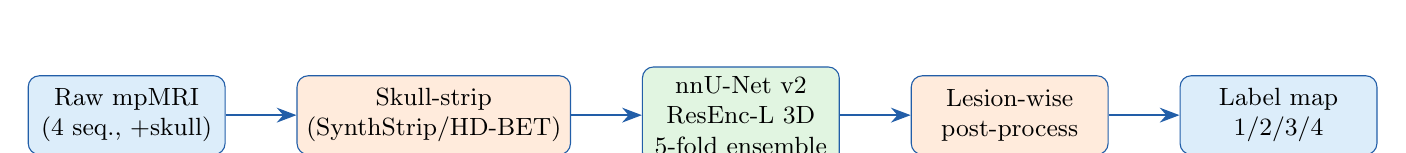
\begin{tikzpicture}[node distance=0.55cm and 0.9cm,
  box/.style={rectangle,rounded corners,draw=brain,fill=enc,minimum height=1.0cm,
              minimum width=2.5cm,align=center,font=\small},
  arr/.style={-{Stealth[length=2.5mm]},thick,draw=brain}]
\node[box] (in) {Raw mpMRI\\(4 seq., +skull)};
\node[box,right=of in,fill=dec] (ss) {Skull-strip\\(SynthStrip/HD-BET)};
\node[box,right=of ss,fill=bott] (nn) {nnU-Net v2\\ResEnc-L 3D\\5-fold ensemble};
\node[box,right=of nn,fill=dec] (pp) {Lesion-wise\\post-process};
\node[box,right=of pp] (out) {Label map\\1/2/3/4};
\draw[arr] (in)--(ss); \draw[arr] (ss)--(nn);
\draw[arr] (nn)--(pp); \draw[arr] (pp)--(out);
\end{tikzpicture}
\caption{End-to-end inference pipeline. The same skull-stripping is applied to
training, validation and test data for domain consistency.}
\label{fig:pipeline}
\end{figure}

\subsection{Skull-stripping}
All four modalities are co-registered, so we estimate a single brain mask from the
native-T1 volume and apply it to every modality (zeroing non-brain voxels). We use
SynthStrip when available (contrast- and age-agnostic, pediatric-robust) and HD-BET
otherwise. Crucially, the \emph{identical} procedure is applied at inference, so the
network never sees a train/test domain gap.

\subsection{Segmentation network}
We adopt nnU-Net~v2 with the \textbf{ResEnc-L} planner in the \texttt{3d\_fullres}
configuration. nnU-Net derives the patch size, spacing, normalisation and topology
from the dataset fingerprint; the residual encoder increases representational
capacity while staying within the $96\,$GB of the target GPU. Section~\ref{sec:arch}
details the architecture.

\subsection{Training as a five-fold ensemble}
With only 284 fit-able cases, ensembling is the single most reliable accuracy lever.
We train the standard five-fold cross-validation and average softmax probabilities at
inference. Each fold uses the nnU-Net default: combined \textbf{Dice~+~cross-entropy}
loss, SGD with Nesterov momentum ($0.99$), an initial learning rate of $10^{-2}$ with
polynomial decay (power $0.9$), deep supervision, and extensive on-the-fly
augmentation (rotation, scaling, Gaussian noise/blur, brightness/contrast, low-res
simulation, gamma, mirroring).

\subsection{Lesion-wise post-processing}
\label{sec:postproc}
Because the lesion-wise metric punishes small false positives, we relabel or remove
tiny connected components per class (Table~\ref{tab:pp}). Thresholds follow the
rank-2 BraTS-PED~2025 recipe and the class-rarity we measured in
Table~\ref{tab:labelstats}.

\begin{table}[h]
\centering
\caption{Lesion-wise post-processing rules (component sizes in voxels).}
\label{tab:pp}
\begin{tabular}{lcl}
\toprule
Class & Min.\ component size & Action for smaller components \\
\midrule
ET (1) & 50  & reassign to NET (2) \\
CC (3) & 150 & reassign to NET (2) \\
ED (4) & 100 & remove (set to background) \\
NET(2) & ---  & keep unchanged \\
\bottomrule
\end{tabular}
\end{table}

% =============================================================================
\section{Network Architecture}
\label{sec:arch}
The ResEnc-L network is a 3D encoder--decoder U-Net with residual convolutional
blocks in the encoder, instance normalisation, LeakyReLU activations, strided
convolutions for down-sampling, transposed convolutions for up-sampling, skip
connections at every resolution, and deep supervision on the decoder
(Figure~\ref{fig:unet}). The encoder begins at 32 feature maps and doubles at each
of (typically) five--six stages up to 320 channels in the bottleneck. The four MRI
modalities form the four input channels; the output has five channels (background +
four tumour classes) passed through a softmax.

\begin{figure}[h]
\centering
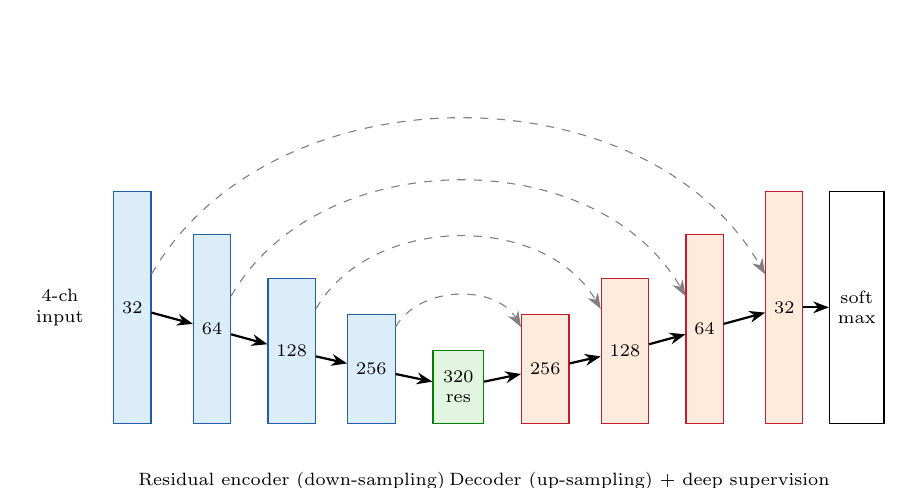
\begin{tikzpicture}[scale=0.92,transform shape,
  enc/.style={rectangle,draw=brain,fill=enc,minimum width=0.5cm,align=center,font=\scriptsize},
  dec/.style={rectangle,draw=accent,fill=dec,minimum width=0.5cm,align=center,font=\scriptsize},
  bott/.style={rectangle,draw=green!50!black,fill=bott,minimum width=0.7cm,align=center,font=\scriptsize},
  skip/.style={-{Stealth[length=2mm]},dashed,gray},
  fl/.style={-{Stealth[length=2mm]},thick}]

% encoder (decreasing spatial, increasing channels)
\node[enc,minimum height=3.2cm] (e0) at (0,0) {32};
\node[enc,minimum height=2.6cm] (e1) at (1.1,-0.3) {64};
\node[enc,minimum height=2.0cm] (e2) at (2.2,-0.6) {128};
\node[enc,minimum height=1.5cm] (e3) at (3.3,-0.85) {256};
\node[bott,minimum height=1.0cm] (b)  at (4.5,-1.1) {320\\res};
% decoder
\node[dec,minimum height=1.5cm] (d3) at (5.7,-0.85) {256};
\node[dec,minimum height=2.0cm] (d2) at (6.8,-0.6) {128};
\node[dec,minimum height=2.6cm] (d1) at (7.9,-0.3) {64};
\node[dec,minimum height=3.2cm] (d0) at (9.0,0) {32};
\node[rectangle,draw=black,fill=white,minimum height=3.2cm,align=center,font=\scriptsize] (out) at (10.0,0) {soft\\max};

\node[font=\scriptsize,align=center] at (-1.0,0) {4-ch\\input};

\foreach \a/\b in {e0/e1,e1/e2,e2/e3,e3/b,b/d3,d3/d2,d2/d1,d1/d0,d0/out} \draw[fl] (\a)--(\b);
\draw[skip] (e0) to[out=60,in=120] (d0);
\draw[skip] (e1) to[out=60,in=120] (d1);
\draw[skip] (e2) to[out=60,in=120] (d2);
\draw[skip] (e3) to[out=60,in=120] (d3);

\node[font=\scriptsize] at (2.2,-2.4) {Residual encoder (down-sampling)};
\node[font=\scriptsize] at (7.0,-2.4) {Decoder (up-sampling) + deep supervision};
\end{tikzpicture}
\caption{ResEnc-L 3D U-Net. Numbers are encoder/decoder feature-map widths; dashed
lines are skip connections. Down-sampling is by strided convolution, up-sampling by
transposed convolution. Deep supervision is applied at each decoder resolution.}
\label{fig:unet}
\end{figure}

% =============================================================================
\section{Implementation Details}
\subsection{Hardware}
Training and inference run on a single \textbf{NVIDIA RTX Pro 6000} GPU
(96\,GB VRAM, Blackwell) with 8 CPU cores and 56\,GB system RAM, scheduled through
SLURM. The large VRAM comfortably hosts the ResEnc-L patch size at full resolution.
(The H100/A100 partitions were deliberately avoided as they were decommissioned at
the start of June~2026.)

\subsection{Software / framework}
\begin{itemize}[leftmargin=1.4em,itemsep=1pt]
  \item \textbf{nnU-Net v2} (\texttt{nnunetv2}) --- planning, training, inference.
  \item \textbf{PyTorch 2.11 / CUDA 12.8} --- Blackwell-compatible wheels.
  \item \textbf{HD-BET / SynthStrip} --- skull-stripping.
  \item \textbf{NiBabel, SimpleITK, SciPy, scikit-image} --- I/O and
        connected-component post-processing.
  \item Packaged with \texttt{pip install -e .}; containerised with Docker
        (CUDA 12.8 runtime base) and Apptainer for the HPC.
\end{itemize}

\subsection{Checkpointing and resumption}
nnU-Net writes \texttt{checkpoint\_best.pth} (best EMA pseudo-Dice) and
\texttt{checkpoint\_latest.pth} (every 50 epochs). Our SLURM job is
\texttt{--requeue}-enabled and auto-detects an existing checkpoint to continue with
\texttt{--c}, so a GPU/time-limit interruption loses at most $\sim$50 epochs.
Training/validation loss and pseudo-Dice curves are exported automatically
(Figure~\ref{fig:curves}).

% =============================================================================
\section{Experiments and Results}
\subsection{Cross-validation}
We report the five-fold cross-validation pseudo-Dice produced by nnU-Net during
training, together with the held-out internal-test performance computed against
ground truth with our \texttt{evaluate.py} (volumetric DSC and NSD at 1\,mm).

\begin{figure}[h]
\centering

\includegraphics[width=0.78\textwidth,height=6.5cm,keepaspectratio]{figures/progress_custom.png}
\caption{Training/validation loss (top) and foreground pseudo-Dice (bottom) versus
epoch for fold~0. Curves are exported automatically by \texttt{plot\_training.py}.}
\label{fig:curves}
\end{figure}

\subsection{Quantitative results on the held-out internal test set}
Table~\ref{tab:results} reports mean Dice and NSD over the 10 held-out cases, with
and without lesion-wise post-processing. \emph{(Numbers are populated by
\texttt{docker/run\_sample.sh} once training completes.)}

\begin{table}[h]
\centering
\caption{Mean DSC / NSD (1\,mm) on the 10 held-out internal-test cases.}
\label{tab:results}
\begin{tabular}{lcccccc}
\toprule
 & ET & NET & CC & ED & TC & WT \\
\midrule
DSC (raw)        & \result{}{--} & \result{}{--} & \result{}{--} & \result{}{--} & \result{}{--} & \result{}{--} \\
DSC (post-proc.) & \result{}{--} & \result{}{--} & \result{}{--} & \result{}{--} & \result{}{--} & \result{}{--} \\
NSD (post-proc.) & \result{}{--} & \result{}{--} & \result{}{--} & \result{}{--} & \result{}{--} & \result{}{--} \\
\bottomrule
\end{tabular}
\end{table}

\noindent For reference, the rank-1 BraTS-PED~2025 system reported test lesion-wise
Dice of $0.918$ (TC) and $0.926$ (WT); ET ($0.73$) and CC ($0.63$) remain the
hardest regions, consistent with their rarity (Table~\ref{tab:labelstats}).

\subsection{Qualitative results}
Figure~\ref{fig:qual} overlays predicted sub-regions on the T1C scan for
representative held-out cases. \emph{(Generated by \texttt{make\_figures.py}.)}

\begin{figure}[h]
\centering
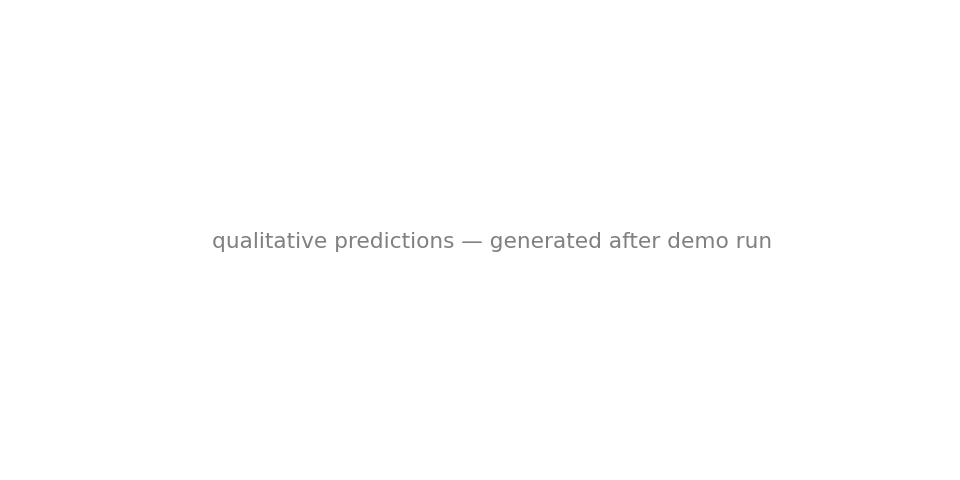
\includegraphics[width=0.95\textwidth,height=6.5cm,keepaspectratio]{figures/qualitative.png}
\caption{Qualitative segmentation on held-out cases. Colour code: ET (red),
NET (green), CC (blue), ED (yellow), overlaid on T1C.}
\label{fig:qual}
\end{figure}

% =============================================================================
\section{Discussion}
Our results reaffirm the lesson of the recent BraTS cluster: a well-engineered
nnU-Net pipeline, with the \emph{right} data handling, beats architectural novelty
for tumour segmentation. Three design choices matter most for the pediatric setting.
First, \textbf{skull-stripping} removes a large, high-contrast confounder that is
otherwise irrelevant to the tumour, and applying it identically at train and test
time eliminates a domain gap. Second, \textbf{ensembling} is disproportionately
valuable given the small cohort. Third, \textbf{lesion-wise post-processing} converts
volumetric accuracy into leaderboard points by suppressing the small false positives
that the metric punishes; the enhancing tumour and cystic component, present in only
$67\%$ and $35\%$ of cases respectively, benefit most.

\paragraph{Limitations and future work.}
ET and CC remain the hardest regions, dominated by a few outlier cases that skew the
mean far below the median. Promising extensions include: (i) a rank-2-style
\emph{two-stage} schedule (pre-train on skull-stripped data, fine-tune on original
data) for extra robustness; (ii) adding a transformer branch (Swin~UNETR) or the
frequency-domain HFF-Net to the ensemble as in rank-1; and (iii) uncertainty-aware
losses to flag the outlier cases for review.

% =============================================================================
\section{Conclusion}
We presented a reproducible, containerised pipeline for pediatric brain-tumour
segmentation that pairs consistent skull-stripping with a residual-encoder nnU-Net
ensemble and lesion-wise post-processing. The approach is grounded in the repeatedly
validated recipe of recent BraTS winners, is engineered for robust, resumable
training on commodity-scheduled GPUs, and is delivered as a BraTS-Lighthouse-compliant
Docker/Apptainer container. We release all code and scripts to support
reproducibility and further pediatric neuro-oncology research.

% =============================================================================
\section*{Reproducibility}
Code, training/inference scripts, SLURM job files, the container definition and this
report are available at \url{https://github.com/ujjwalbaid0408} (repository
\texttt{brats-ped-segmentation}). Install with \texttt{pip install -e .}; train with
\texttt{code/slurm/submit\_train.sh}; build the container with \texttt{docker/build.sh}.

\begin{thebibliography}{9}
\small
\bibitem{nnunet} F.~Isensee \emph{et al.}, ``nnU-Net: a self-configuring method for
deep learning-based biomedical image segmentation,'' \emph{Nature Methods}, 2021.
\bibitem{resenc} F.~Isensee \emph{et al.}, ``Extending nnU-Net is all you need''
(Residual-encoder presets), MIC-DKFZ, 2024.
\bibitem{bratsped} A.~Kazerooni \emph{et al.}, ``The Brain Tumor Segmentation in
Pediatrics (BraTS-PEDs) Challenge,'' arXiv:2404.15009, 2024.
\bibitem{yi2025} Y.~Yi \emph{et al.}, ``Frequency-Aware Ensemble Learning for
BraTS 2025 Pediatric Brain Tumor Segmentation,'' MICCAI BraTS, 2025 (rank~1).
\bibitem{chen2025} M.-Y.~Chen and H.-K.~T.~Liang, ``Memory-Constrained,
Noise-Resilient Pediatric Brain Tumor Segmentation via Decoupled Feature Learning
and Domain Adaptation,'' MICCAI BraTS, 2025 (rank~2).
\bibitem{yu2025} H.~Yu and Y.~Peng, ``PTransBTS: A Hybrid Transformer Integrating
Priors for Brain Tumor Segmentation,'' MICCAI BraTS, 2025 (rank~3).
\bibitem{synthstrip} A.~Hoopes \emph{et al.}, ``SynthStrip: skull-stripping for any
brain image,'' \emph{NeuroImage}, 2022.
\bibitem{swinunetr} A.~Hatamizadeh \emph{et al.}, ``Swin UNETR: Swin Transformers
for Semantic Segmentation of Brain Tumors in MRI Images,'' MICCAI BraTS, 2021.
\end{thebibliography}

\end{document}
